\chapter{Patterning in Synthetic Bacterial Colonies} \label{chapter3}
%Chapter one describes how systems might be more robust for patterning than linear stability analysis predicts, and that we should look for other analytical solutions when considering patterning.
%It also studied how growth and boundaries might change the patterning outcome.
%
%In chapter 2 the patterning capabilities of the gene circuit engineered in ~\cite{Tica2020} were studied.
%It was shown that patterns can arise from this circuit.
%Certain parameter regimes are more robust for patterning, such as matching transfer functions, adding aTc,DAPG or slowing $D_{V}$ diffusion.
%Finally, in chapter 2 the circuit was parametrised using the model under liquid culture experiments which have followed the circuit tuning guidance to optimise Turing robustness.
%%
%Following chapter 2 insights, I carried out spatial experiments were carried out with the optimal tuning conditions.
%In this chapter, chapter 1 and chapter 2 knowledge is combined and spatial experiments  based on our previous work.


In this chapter, the focus is on experiments and modelling of the gene circuit in a bacterial biofilm.
In this thesis, initial experiments on small colonies are carried out where concentric rings appear. Following this, further experiments by Isalan Group are caried out to further explore these rings.
Then, pattern forming biofilms are replicated using a model and mechanism is understood.
%
%The aim is to predict pattern formation under the chosen spatial setup which are growing colonies.
%Additionally, for the patterns obtain, the aim is to obtain mechanistic insights of what the patterns can do.
%This is done first with the general parameter distribution from the literature to explore the overall potential of the circuit in bacterial colonies.
%Then, is done in the parametrised distributions to get more specific insights into the mechanisms in the regions we find ourselves in and to have a more predictable model.

\section{Experimental rings in small colonies with high aTc}\label{Rings in small colonies with high aTc}
In the previous chapter, certain conditions which could affect robustness for Turing pattern formation are found.
As already shown, the circuit components were matched by Jure Tica and Tong Zhu (see Fig~\ref{fig:dose_response_experimental}) to improve robustness as seen in Fig.~\ref{fig:balancing_robustness}.
In this section, I investigate the circuit in a biofilm using confocal microscopy under those optimal Turing conditions.
More specifically, I look at how the biofilm fluorescent patterns change with different levels of aTc in small colonies

MK01 \textit{E.coli} cells were transformed using electroporation (Section~\ref{electroporation}) with the full circuit.
This involved the introduction of 4 plasmids with the three nodes and the regulator cassette as seen in Fig.~\ref{fig:synthetic circuit_chapter2} and Table~\ref{tab:plasmid table} into our \textit{E.coli} cells.
For this, the cells were then plated in 6 well MatTek plates and grew as individual colonies which are radially growing biofilms.
These growing colonies are then imaged using confocal microscopy.
Confocal microscopy is a type of fluorescence microscopy used to image thicker objects, where the beam of light focuses on one depth level, meaning you can get a single z plane of fluorescence.
This way we can obtain a 2D fluorescence pattern steaming from a single focal plane of the colony ~\parencite{semwogerere2005confocal}.
 Detailed methods on colony plating and microscopy can be found in Section~\ref{microscopy}
Red and green channels were imaged to detect mCherry and GFP as seen in Fig.~\ref{rgchannels}A,B.
These channels can then be superposed to get a GFP-mCherry combined reading (Fig.~\ref{rgchannels}C)
\begin{figure}[H]

    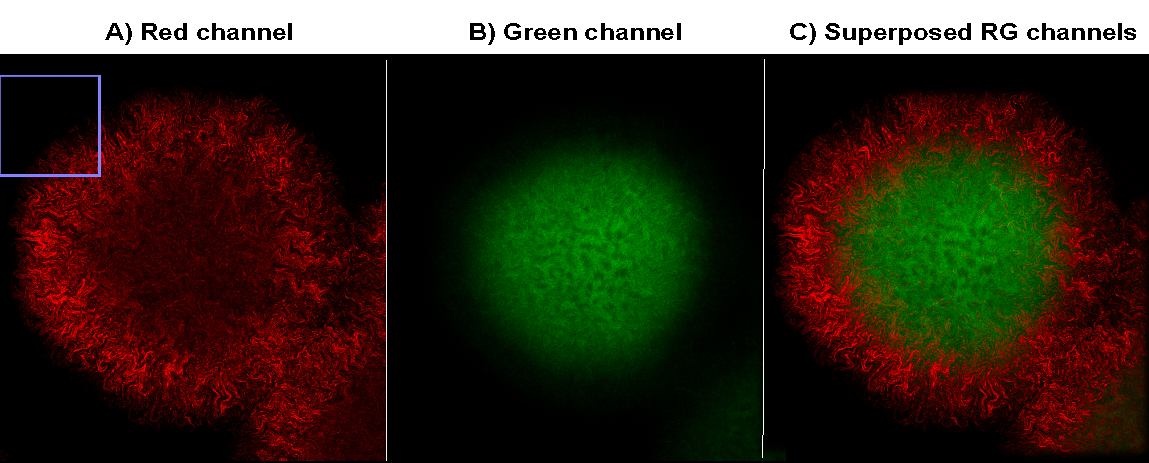
\includegraphics[width=1\textwidth]{chapters/Chapter 3/rgchannels}
    \caption{add}
    \label{rgchannels}
\end{figure}

To test the impact of aTc on the patterning of the circuit, we prepared the agar on the MaTek plates with different levels of aTc, ranging from 0 to $10^1 \mu M$.
Different colony patterns arise from this aTc walk as seen in Fig.~\ref{atcwalk_timeseries_confocal}A.
The colonies exhibiting more spatially heterogeneous behaviour are those with high aTc ($10^1 \mu M$).
This high aTc condition is further explored by imaging every day.
In Fig.~\ref{atcwalk_timeseries_confocal}B, we see how over time, the center of the colony oscillates from black to red to green.
As this happens, rings get added from the center as in~\cite{Konow2019}'s inner ring addition mechanism.
The final snapshot (64h) shows green, red, green, red progression steaming from the center.

\begin{figure}[H]

    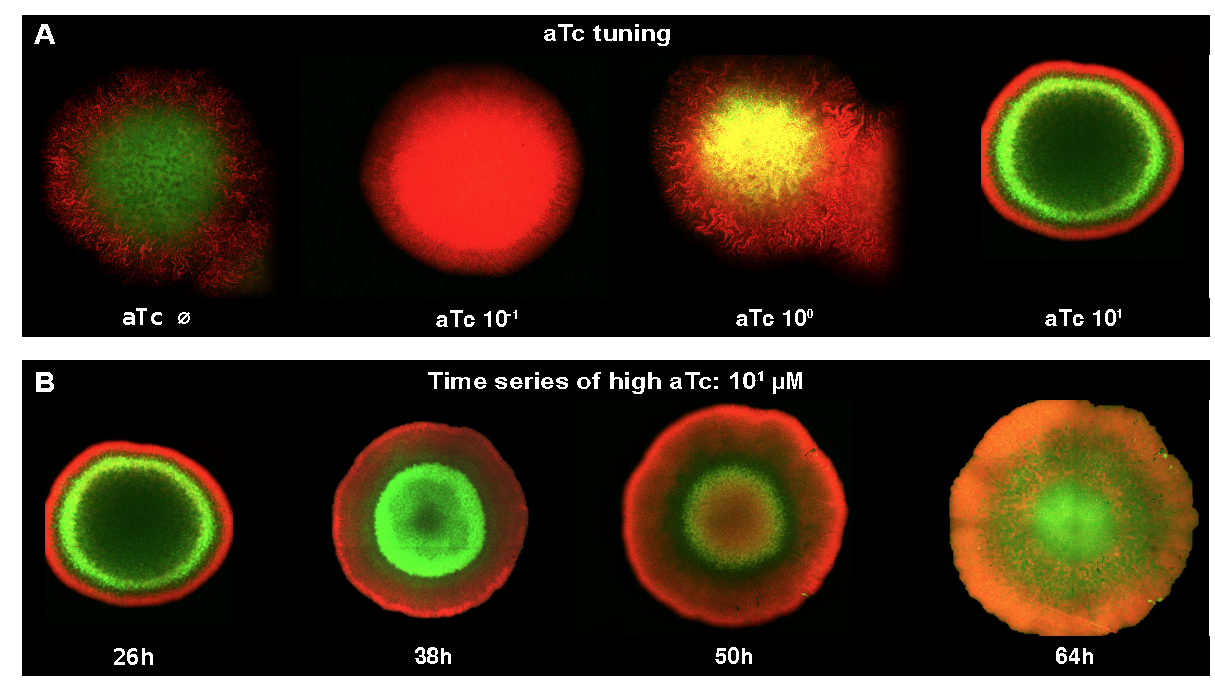
\includegraphics[width=1\textwidth]{chapters/Chapter 3/atcwalk_timeseries_confocal}
    \caption{\textbf{Confocal images of small colonies with gene circuit 3943}. A) Colonies with different atc conditions at time 26h: no aTc $10^{-1} \mu M,10^{0} \mu M,10^{1} \mu  $. B) Time series of single colony with high aTc condition ($10^1 \mu M$).}
    \label{atcwalk_timeseries_confocal}
\end{figure}

Following this work, Jure Tica, Tong Zhu and Georg Wachter continued studying this synthetic patterning system more in depth.
Two routes were followed.
The first one involved specific shaped domains achieved by imprinting the agar with bacteria using shaped objects (Fig.~\ref{shmoo}).
The aim was to understand how the pattern adapts under different shaped domains.
The second route, and most explored, involved larger colonies to determine whether more repeats would form in a Turing-like behaviour.
This was achieved by carefully diluting the sample and plating a single colony without any neighbours.

\section{Modelling framework for synthetic circuit in bacterial tissues}
Most theoretical studies which involve Turing patterns, numerically simulate their system using square domains with no-flux or periodic boundary conditions.
However, these numerical domains are often not biologically realistic.
For exampled, the system we have developed experimentally involves more specific conditions including shaped domains, stochastic growth and absorbing boundary conditions.
To have a predictable model of our experimental system, the numerical solver had to be adapted to include such domain characteristics.

\subsection{Alternating Direction Implicit Method with defined domains}\label{Alternating Direction Implicit Method with defined domains}
All simulations in this chapter are performed in a \acrshort{2D} space to match the \acrshort{2D} focal plane captured by the confocal microscopy.
For this purpose, the numerical solver schema  \acrfull{ADI} is used.
This numerical solver produces a 2D space solution in time for the $n$ number of species of the model.
This method is chosen over \acrshort{CN} used in the previous chapter, as it is more efficient to solve 2D problems due to the matrix diagonalisation (See Section~\ref{numerical_methods}). More specific details of ADI can be found in Section~\ref{ADI}.



ADI is originally defined to solve square domains.
To integrate our specific domains with the solver, a masking system is used where a "shape matrix" is passed containing the shape of the domain.
The "shape matrix" has is a boolean matrix of $IxJ$ size which contains information on the location of the cells.
1's determine cells, while 0's determine agar.
When passing this matrix to the solver, the algorithm computes reaction and diffusion terms in 1 positions while it only computes diffusion in 0's.
Fig.~\ref{mask}~right shows the "shape matrix" where 1's are black and 0's are white.
Additionally, this figure shows what functions are computed in which regions.
How the "shape matrix" is defined depends on the experimental setup.
Using this masking method, we will obtain a solution for the $n$ number of species of our model, in time and in space, within the biofilm.

\begin{figure}[H]
    \centering

    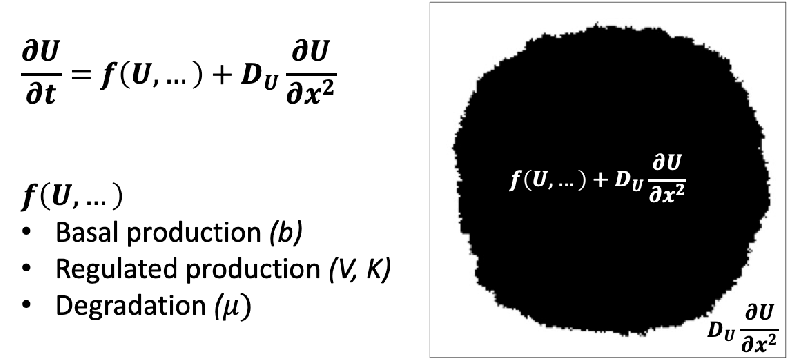
\includegraphics[width=0.9\textwidth]{chapters/Chapter 3/mask}
    \caption{a}
    \label{mask}
\end{figure}

\subsection{Static Shaped domains}
Following the small rings produced in this thesis, Tong Zhu from the Isalan Lab started experimenting with non-circular domains.
Specific shapes were obtained by imprinting the agar with bacteria using shaped objects.
Fig.~\ref{shmoo}A shows the resulting biofilm after impregnating the agar with bacteria using the edge of a glass coverslip. %TODO ref figure
In this thesis, the biofilm shape is replicated by using a "shape matrix" derived from the microscopy image Fig.~\ref{shmoo}B.
This is done through image recognition on the microscopy snapshots to detect areas with cells (See Section~\ref{Tissue area recognition}).


\begin{figure}[H]
    \centering

    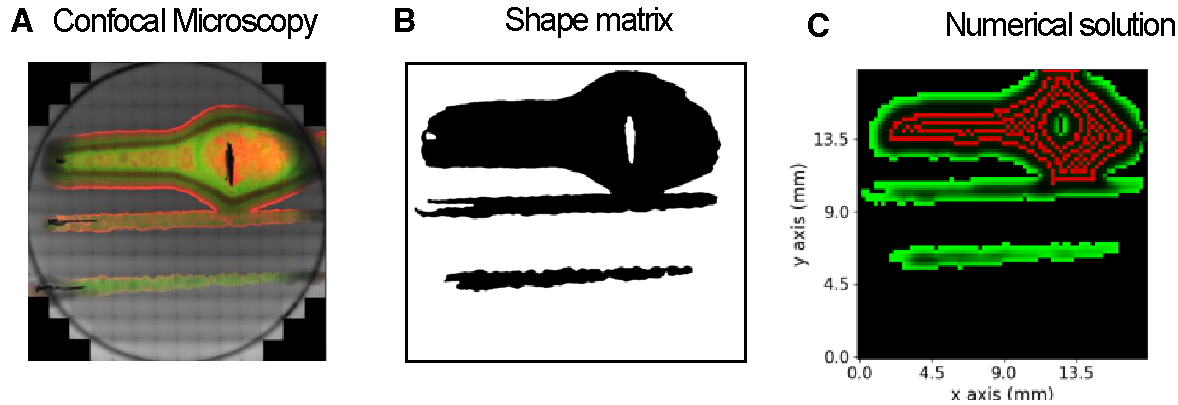
\includegraphics[width=1\textwidth]{chapters/Chapter 3/shmoo}
    \caption{}
    \label{shmoo}
\end{figure}
Using the masking method with ADI explained in ~\ref{Alternating Direction Implicit Method with defined domains}, a numerical solution was computed within the defined biofilm.
The PDE system used is the six-equation model (Eq.~\ref{[6 equation proteins]}), which describes synthetic circuit 3954, using a Turing parameter set found through linear stability analysis.
The numerical solution is shown in Fig.~\ref{shmoo}C as a superposition of the red and green channel.
Details on the plotting the numerical solution of the 6-equation as a red-green image like confocal microscopy can be found in Section~\ref{Plotting superposed numerical solution as confocal microscopy results}

\subsection{Growing colony with cellular automaton}
Most of the work we carried out experimentally to explore the system was done in bacterial colonies.
These colonies are radially growing biofilms with stochastic cell division.
Therefore, the static image recognition method used above is not suitable as we do not have time-series confocal data for most samples to create a dynamic "shape matrix".
To recreate the dynamic behaviour of the colony growing, a stochastic growth model was developed using a cellular automaton.

A cellular automaton is a discrete model of computation constructed with a few basic rules ~\parencite{gardner1970mathematical}, which can accurately describe how the shape of the bacterial colony evolves over time.
As the "shape matrix", the cellular automaton consists of a boolean 2-dimensional matrix, where grid-points can be in a cell (1) or agar (0) state.
This boolean matrix evolves over time when the following three rules are applied: If an cell (1) grid-point has any agar (0) neighbours, it will divide into the neighbouring agar (0) gridpoint with a probability $p_{d}$.
No cell death (1 to 0 transition) is permitted.
Newborn cells inherit the full concentration of their mother cells.
This last assumption is taken as mRNA transcript homeostasis ensures concentration of mRNAs is mantained at cell division and as cell size increases by scaling between transcription rates and cell size ~\parencite{berry2022mechanisms,volteras2023global}.
Because we are modelling protein concentration, we can then assume that mRNA concentration is linearly correlated with protein concentration for synthetic genes like ours.
If some dilution occurs, this can be accounted for in the degradation terms of the PDE model.

To model a single colony, a 0's matrix is initialised with a 1 in the middle, describing the first cell as it occurs in single cell colonies.
When the cellular automaton rules are applied to this initial matrix, a circular cell domain starts growing stochasticly, resembling a bacterial colony (See Fig.\ref{cas}A-B).
The division process consists of a probabilistic process where division occurs or not based on a probability of division ($p_{d}$).
The division process is iteratively applied to the matrix until the final time (T) is reached.
The computation is applied every ‘m’ hours, so
\begin{equation}
        T = \sum_{n=1}^{T/m} m\cdot n
\end{equation}

e.g. if $m=0.2$ at $T=0.2, 0.4, 0.6 \ldots etc$ .
The growth rate can be tuned by increasing the probability of division ($p_d$) or decreasing $m$, so it matches the experimental growth rates. Furthermore, different $p_d$’s can be applied to different regions of the matrix to achieve faster growing subregions within the colony (See Fig.~\ref{cas}C). Finally, to simulate two colonies, two 1’s are placed at a distance (See Fig.~\ref{cas}D).

\begin{figure}[H]
    \centering

    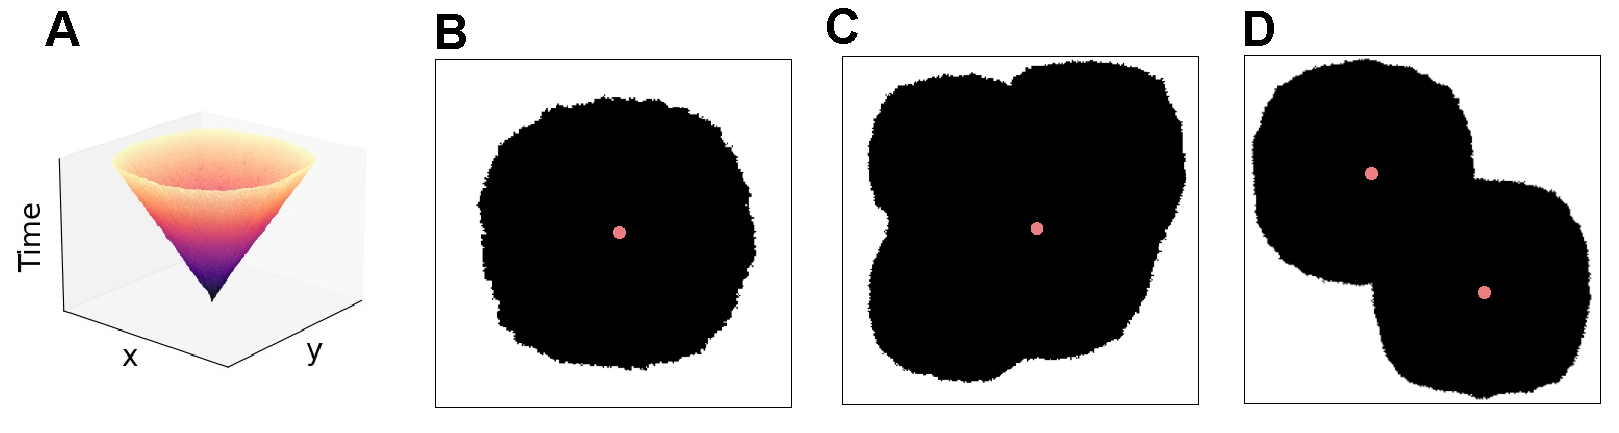
\includegraphics[width=1\textwidth]{chapters/Chapter 3/cas}
    \caption{}
    \label{cas}
\end{figure}

The masks obtained can be used to compute the solution of the PDE in the biofilm.
Taking an arbitrary parameter set, this method produces a numerical result similar to that of the colonies obtained in Section~\ref{Rings in small colonies with high aTc}.
The comparison can be seen in Fig.~\ref{small colony experiment vs model} where the red edge with green center is reproduced.
This pattern is commonly seen throughout, as it stems from the boundary effects at the edge of the colony which is capture by the masking method.
At the edge of the colony, there is a depletion of diffusers as they leak out onto the agar.
By looking at the circuit (Fig.~\ref{fig:synthetic circuit_chapter2}), we can observe that diffusors are direct GFP activators and mCherry inhibitors.
Therefore, as they get depleted, red is produced and green decays. 
\begin{figure}[H]
    \centering

    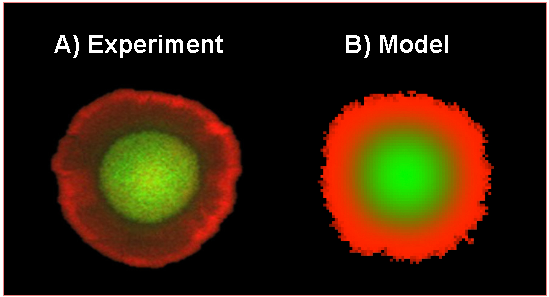
\includegraphics[width=0.6\textwidth]{chapters/Chapter 3/small colony experiment vs model}
    \caption{}
    \label{small colony experiment vs model}
\end{figure}

\section{Colony pattern dynamics in parameter space searches}

The experimental work in this thesis produced the first rings observed in the system, where small colonies were used (Section~\ref{Rings in small colonies with high aTc}).
Following this, experiments were carried out in larger colonies by Jure Tica, Tong Zhu and Georg Wachter from the Isalan Lab.
From here onwards, experimental images were produced by them unless otherwise stated.
A wide variety of patterns were produced by growing larger colonies.


\subsection{Circuit exploration in literature-based distribution}
In parallel to microscopy work, the model predicted a wide variety of patterns could be produced in different dynamical regimes, which matched the experimental variability.
This was shown by exploring the parameter space of our circuit within literature-based ranges.
The distribution used is described in Section~\ref{Definition of parameter space based on literature parametrisation} and more specifically Table~\ref{tab:literature param distributions}.
In this exploration, first linear stability analysis was carried out and outputs were classified following linear stability classification in Fig.~\ref{fig:dispersions}.
The frequencies in parameter space of the linear stability solutions are shown in Fig.~\ref{system_class_frequencies}.

\begin{figure}[H]
    \centering

    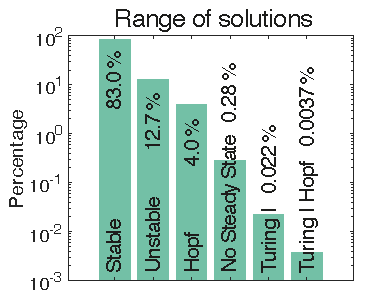
\includegraphics[width=0.6\textwidth]{chapters/Chapter 3/system_class_frequencies}
    \caption{}
    \label{system_class_frequencies}
\end{figure}

Examples of different linear stability analysis outputs were solved numerically, masked by a growing colony obtained with the cellular automata algorithm.
The different final pattern snapshots and time-series can be seen in Fig~\ref{system_class_simulations}.
A wide variety of patterns and dynamics is observed.
Hopf solutions produce oscillatory patterns, some ring-like and some spot-like.
Finally, Stable, Unstable and Systems with no steady states produce more homogeneous type solutions, which may be stationary or oscillatory.
It is important to add that Turing I Hopf solutions seem to produce patterns more robustly in this chapter than in chapter 1. %TODO add maye in discussion
All of patterns shown are single steady state systems so we can understand the individual and isolated behaviour of that dynamical system.
However some interesting multistable systems are present such as the Turing-Hopf-Unstable system shown in FigX.
\begin{figure}[H]
    \centering

    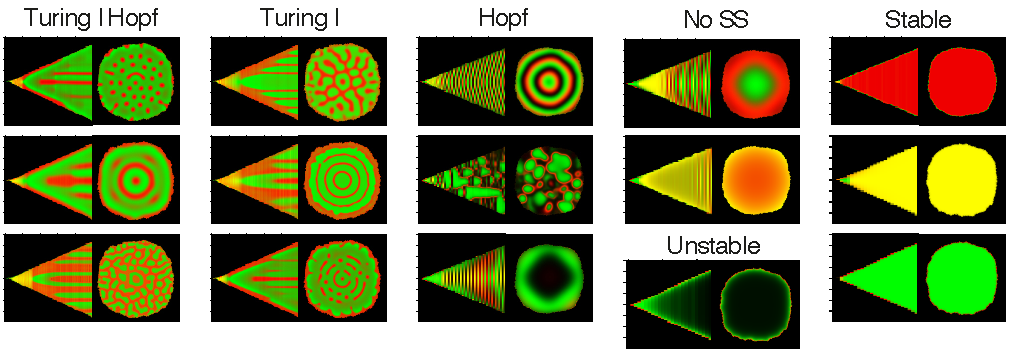
\includegraphics[width=1\textwidth]{chapters/Chapter 3/system_class_simulations}
    \caption{}
    \label{system_class_simulations}
\end{figure}




\subsection{Circuit exploration in liquid-culture fits distribution}

\section{Elucidating mechanisms through experiment controls}
\subsection{Physical controls}
\subsubsection{Size}
\subsubsection{Boundary}
\subsubsection{Temperature}

\subsection{Genetic controls}
\subsubsection{Experimental deletions}
\subsubsection{Model deletions}
%experimental node deletions
%lsa and numerical controls prove no patterns
%cold shock controls + %timeseries
\section{Discussion}


%\section{Modelling bacterial colonies}
%\subsection{openboundary circle shape growth noise}
%\section{Explore patterning potential}
%\subsection{general params}
%\subsection{parametrised params}
